
\begin{figure}
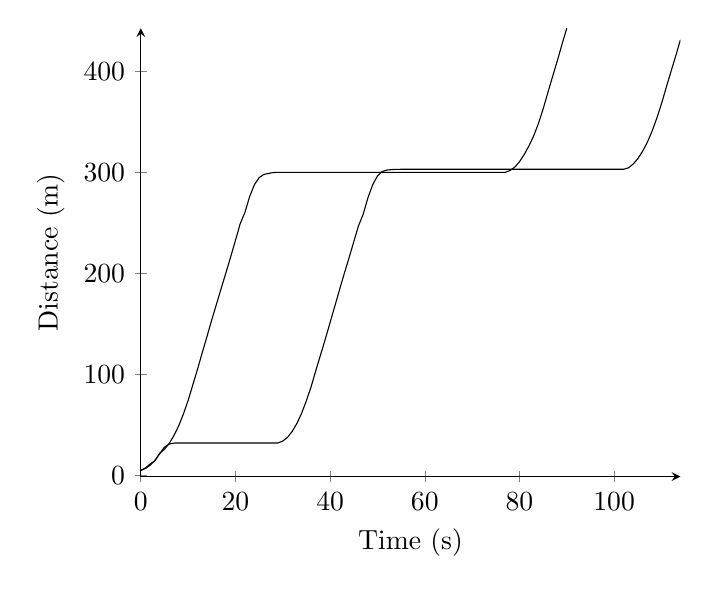
\begin{tikzpicture}
\begin{axis}[
legend style={anchor=west},
axis x line=bottom,
axis y line=left,
ymin=-1,
xlabel=Time (s),
ylabel=Distance (m),
]
\addplot[] coordinates {
(0, 5.1)
(1, 7.03027883099)
(2, 10.2461998621)
(3, 15.0877679488)
(4, 21.6020636184)
(5, 28.0573987335)
(6, 31.1842445499)
(7, 32.1649788726)
(8, 32.2220131933)
(9, 32.2557313773)
(10, 32.2658975558)
(11, 32.2658975558)
(12, 32.2658975558)
(13, 32.2658975558)
(14, 32.2658975558)
(15, 32.2658975558)
(16, 32.2658975558)
(17, 32.2658975558)
(18, 32.2658975558)
(19, 32.2658975558)
(20, 32.2658975558)
(21, 32.2658975558)
(22, 32.2658975558)
(23, 32.2658975558)
(24, 32.2658975558)
(25, 32.2658975558)
(26, 32.2658975558)
(27, 32.2658975558)
(28, 32.2658975558)
(29, 32.2658975558)
(30, 34.1152390342)
(31, 37.817931568)
(32, 43.8459610466)
(33, 51.6936293304)
(34, 61.9049137678)
(35, 74.2607836814)
(36, 88.141345248)
(37, 104.273731818)
(38, 119.778422953)
(39, 135.344708661)
(40, 151.647076932)
(41, 167.850997959)
(42, 184.225626814)
(43, 200.169603079)
(44, 215.566654904)
(45, 231.571414259)
(46, 247.309865114)
(47, 258.941168569)
(48, 275.254587177)
(49, 287.987360175)
(50, 296.655948886)
(51, 301.029113454)
(52, 302.4956904)
(53, 302.971433083)
(54, 303.198501255)
(55, 303.254320406)
(56, 303.266891404)
(57, 303.266891404)
(58, 303.266891404)
(59, 303.266891404)
(60, 303.266891404)
(61, 303.266891404)
(62, 303.266891404)
(63, 303.266891404)
(64, 303.266891404)
(65, 303.266891404)
(66, 303.266891404)
(67, 303.266891404)
(68, 303.266891404)
(69, 303.266891404)
(70, 303.266891404)
(71, 303.266891404)
(72, 303.266891404)
(73, 303.266891404)
(74, 303.266891404)
(75, 303.266891404)
(76, 303.266891404)
(77, 303.266891404)
(78, 303.266891404)
(79, 303.266891404)
(80, 303.266891404)
(81, 303.266891404)
(82, 303.266891404)
(83, 303.266891404)
(84, 303.266891404)
(85, 303.266891404)
(86, 303.266891404)
(87, 303.266891404)
(88, 303.266891404)
(89, 303.266891404)
(90, 303.266891404)
(91, 303.266891404)
(92, 303.266891404)
(93, 303.266891404)
(94, 303.266891404)
(95, 303.266891404)
(96, 303.266891404)
(97, 303.266891404)
(98, 303.266891404)
(99, 303.266891404)
(100, 303.266891404)
(101, 303.266891404)
(102, 303.266891404)
(103, 304.656183902)
(104, 308.359158456)
(105, 313.759282629)
(106, 321.036005915)
(107, 329.949694843)
(108, 340.818941692)
(109, 353.69262032)
(110, 368.123942493)
(111, 384.195583273)
(112, 399.995180221)
(113, 415.389461394)
(114, 431.516021523)
};
\addplot[] coordinates {
(0, 5.1)
(1, 7.50789333591)
(2, 11.5203682661)
(3, 14.6128220973)
(4, 22.0909060489)
(5, 26.098272735)
(6, 31.6820746399)
(7, 39.5424169562)
(8, 49.1243511638)
(9, 60.7756028792)
(10, 74.2720514203)
(11, 89.8649550296)
(12, 105.416646057)
(13, 121.923336792)
(14, 137.811080644)
(15, 154.253574576)
(16, 169.842771461)
(17, 185.478548748)
(18, 200.955924864)
(19, 216.661877651)
(20, 232.807943091)
(21, 249.353236828)
(22, 260.444440759)
(23, 276.259433101)
(24, 287.962063582)
(25, 294.977898282)
(26, 298.17770374)
(27, 299.173168836)
(28, 300.059183688)
(29, 300.189199925)
(30, 300.245316171)
(31, 300.261893273)
(32, 300.261893273)
(33, 300.261893273)
(34, 300.261893273)
(35, 300.261893273)
(36, 300.261893273)
(37, 300.261893273)
(38, 300.261893273)
(39, 300.261893273)
(40, 300.261893273)
(41, 300.261893273)
(42, 300.261893273)
(43, 300.261893273)
(44, 300.261893273)
(45, 300.261893273)
(46, 300.261893273)
(47, 300.261893273)
(48, 300.261893273)
(49, 300.261893273)
(50, 300.261893273)
(51, 300.261893273)
(52, 300.261893273)
(53, 300.261893273)
(54, 300.261893273)
(55, 300.261893273)
(56, 300.261893273)
(57, 300.261893273)
(58, 300.261893273)
(59, 300.261893273)
(60, 300.261893273)
(61, 300.261893273)
(62, 300.261893273)
(63, 300.261893273)
(64, 300.261893273)
(65, 300.261893273)
(66, 300.261893273)
(67, 300.261893273)
(68, 300.261893273)
(69, 300.261893273)
(70, 300.261893273)
(71, 300.261893273)
(72, 300.261893273)
(73, 300.261893273)
(74, 300.261893273)
(75, 300.261893273)
(76, 300.261893273)
(77, 300.261893273)
(78, 302.069121979)
(79, 305.284997969)
(80, 310.721819914)
(81, 317.89433831)
(82, 326.410220237)
(83, 336.318031188)
(84, 348.547078494)
(85, 362.974308313)
(86, 379.262095475)
(87, 395.100215314)
(88, 410.737653287)
(89, 427.240096836)
(90, 442.94596841)
};

\end{axis}
\end{tikzpicture}
\label{tik:distance:0:16}
\caption{0 percent diving with GSC on route $16$}
\end{figure}
